\hypertarget{interfaceCqrs_1_1Events_1_1IEventHandler}{}\section{Cqrs.\+Events.\+I\+Event\+Handler$<$ T\+Authentication\+Token, T\+Target, in in T\+Event $>$ Interface Template Reference}
\label{interfaceCqrs_1_1Events_1_1IEventHandler}\index{Cqrs.\+Events.\+I\+Event\+Handler$<$ T\+Authentication\+Token, T\+Target, in in T\+Event $>$@{Cqrs.\+Events.\+I\+Event\+Handler$<$ T\+Authentication\+Token, T\+Target, in in T\+Event $>$}}


Responds to or \char`\"{}\+Handles\char`\"{} a {\itshape T\+Event} .  


Inheritance diagram for Cqrs.\+Events.\+I\+Event\+Handler$<$ T\+Authentication\+Token, T\+Target, in in T\+Event $>$\+:\begin{figure}[H]
\begin{center}
\leavevmode
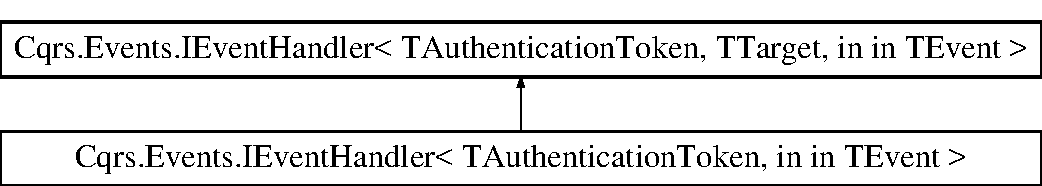
\includegraphics[height=2.000000cm]{interfaceCqrs_1_1Events_1_1IEventHandler}
\end{center}
\end{figure}


\subsection{Detailed Description}
Responds to or \char`\"{}\+Handles\char`\"{} a {\itshape T\+Event} . 


\begin{DoxyTemplParams}{Template Parameters}
{\em T\+Authentication\+Token} & The Type of the authentication token.\\
\hline
{\em T\+Target} & The Type of the object that is targeted that needs concurrency.\\
\hline
{\em T\+Event} & The Type of I\+Event$<$\+T\+Authentication\+Token$>$ that can be handled.\\
\hline
\end{DoxyTemplParams}
\begin{Desc}
\item[Type Constraints]\begin{description}
\item[{\em T\+Event} : {\em \hyperlink{interfaceCqrs_1_1Events_1_1IEvent}{I\+Event}$<$T\+Authentication\+Token$>$}]\end{description}
\end{Desc}
